\section{Date: 2026-07-28}
\noindent \textbf{Series ID: CUUSX100SA0L1E} 

\noindent This series is titled Consumer Price Index for All Urban Consumers: All Items Less Food and Energy in Northeast - Size Class B/C and has a frequency of Semiannual. The units are Index Dec 1997=100 and the seasonal adjustment is Not Seasonally Adjusted.The observation start date is 1998-01-01 and the observation end date is 2026-01-01.The popularity of this series is 1. \\ 

\noindent \textbf{Series ID: CWSR0000SAS4} 

\noindent This series is titled Consumer Price Index for All Urban Wage Earners and Clerical Workers: Transportation Services in U.S. City Average and has a frequency of Monthly. The units are Index 1982-1984=100 and the seasonal adjustment is Seasonally Adjusted.The observation start date is 1956-01-01 and the observation end date is 2026-06-01.The popularity of this series is 1. \\ 

\subsection{Raw Regression}
\noindent Regresses the two series against each other directly. A significant result here can come just as easily from both series sharing a long-run trend as from any real relationship.

\begin{center}
\begin{tabular}{lclc}
\toprule
\textbf{Dep. Variable:}              & value\_fred\_CWSR0000SAS4 & \textbf{  R-squared:         } &     0.974   \\
\textbf{Model:}                      &            OLS            & \textbf{  Adj. R-squared:    } &     0.973   \\
\textbf{Method:}                     &       Least Squares       & \textbf{  F-statistic:       } &     2037.   \\
\textbf{Date:}                       &      Tue, 28 Jul 2026     & \textbf{  Prob (F-statistic):} &  3.80e-45   \\
\textbf{Time:}                       &          13:25:41         & \textbf{  Log-Likelihood:    } &   -227.11   \\
\textbf{No. Observations:}           &               57          & \textbf{  AIC:               } &     458.2   \\
\textbf{Df Residuals:}               &               55          & \textbf{  BIC:               } &     462.3   \\
\textbf{Df Model:}                   &                1          & \textbf{                     } &             \\
\textbf{Covariance Type:}            &         nonrobust         & \textbf{                     } &             \\
\bottomrule
\end{tabular}
\begin{tabular}{lcccccc}
                                     & \textbf{coef} & \textbf{std err} & \textbf{t} & \textbf{P$> |$t$|$} & \textbf{[0.025} & \textbf{0.975]}  \\
\midrule
\textbf{const}                       &    -174.8164  &       10.353     &   -16.886  &         0.000        &     -195.564    &     -154.069     \\
\textbf{value\_fred\_CUUSX100SA0L1E} &       3.3910  &        0.075     &    45.134  &         0.000        &        3.240    &        3.542     \\
\bottomrule
\end{tabular}
\begin{tabular}{lclc}
\textbf{Omnibus:}       &  1.760 & \textbf{  Durbin-Watson:     } &    0.172  \\
\textbf{Prob(Omnibus):} &  0.415 & \textbf{  Jarque-Bera (JB):  } &    0.997  \\
\textbf{Skew:}          &  0.247 & \textbf{  Prob(JB):          } &    0.607  \\
\textbf{Kurtosis:}      &  3.420 & \textbf{  Cond. No.          } &     813.  \\
\bottomrule
\end{tabular}
%\caption{OLS Regression Results}
\end{center}

Notes: \newline
 [1] Standard Errors assume that the covariance matrix of the errors is correctly specified.

\begin{figure}
\centering
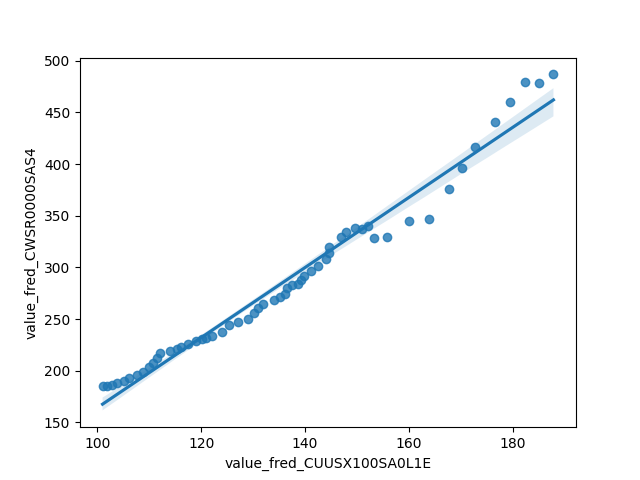
\includegraphics[scale = 0.9]{plots/plot_2026-07-28.png}
\caption{Raw Regression Plot for 2026-07-28}
\end{figure}
\newpage
\subsection{Detrended Regression}
\noindent Regresses the residuals of each series after removing its own linear time trend, so a shared trend can no longer drive the result on its own. A relationship that stays significant here is better evidence of a genuine link between the two series.

\begin{center}
\begin{tabular}{lclc}
\toprule
\textbf{Dep. Variable:}                         & value\_fred\_CWSR0000SAS4\_detrended & \textbf{  R-squared:         } &     0.841   \\
\textbf{Model:}                                 &                 OLS                  & \textbf{  Adj. R-squared:    } &     0.838   \\
\textbf{Method:}                                &            Least Squares             & \textbf{  F-statistic:       } &     290.1   \\
\textbf{Date:}                                  &           Tue, 28 Jul 2026           & \textbf{  Prob (F-statistic):} &  1.35e-23   \\
\textbf{Time:}                                  &               13:25:41               & \textbf{  Log-Likelihood:    } &   -212.21   \\
\textbf{No. Observations:}                      &                    57                & \textbf{  AIC:               } &     428.4   \\
\textbf{Df Residuals:}                          &                    55                & \textbf{  BIC:               } &     432.5   \\
\textbf{Df Model:}                              &                     1                & \textbf{                     } &             \\
\textbf{Covariance Type:}                       &              nonrobust               & \textbf{                     } &             \\
\bottomrule
\end{tabular}
\begin{tabular}{lcccccc}
                                                & \textbf{coef} & \textbf{std err} & \textbf{t} & \textbf{P$> |$t$|$} & \textbf{[0.025} & \textbf{0.975]}  \\
\midrule
\textbf{const}                                  &   -1.098e-11  &        1.350     & -8.13e-12  &         1.000        &       -2.706    &        2.706     \\
\textbf{value\_fred\_CUUSX100SA0L1E\_detrended} &       5.2535  &        0.308     &    17.033  &         0.000        &        4.635    &        5.872     \\
\bottomrule
\end{tabular}
\begin{tabular}{lclc}
\textbf{Omnibus:}       &  3.612 & \textbf{  Durbin-Watson:     } &    0.292  \\
\textbf{Prob(Omnibus):} &  0.164 & \textbf{  Jarque-Bera (JB):  } &    2.762  \\
\textbf{Skew:}          & -0.345 & \textbf{  Prob(JB):          } &    0.251  \\
\textbf{Kurtosis:}      &  3.828 & \textbf{  Cond. No.          } &     4.38  \\
\bottomrule
\end{tabular}
%\caption{OLS Regression Results}
\end{center}

Notes: \newline
 [1] Standard Errors assume that the covariance matrix of the errors is correctly specified.

\begin{figure}
\centering
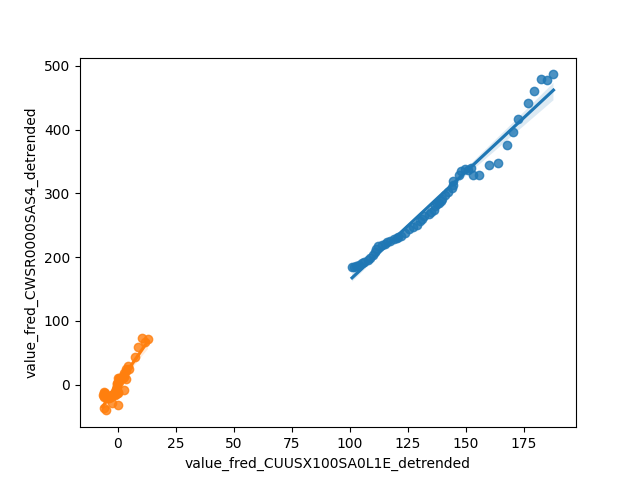
\includegraphics[scale = 0.9]{plots/plot_2026-07-28_detrended.png}
\caption{Detrended Regression Plot for 2026-07-28}
\end{figure}
\newpage
